% documentclass options:
% a4paper | letterpaper | ...  - paper size
% 10pt | 11pt | 12pt           - font size
% onecolumn | twocolumn        - toggle two columns
% titlepage | notitlepage      - toggle title page
% oneside | twoside            - toggle styling for two-side printing
% landscape                    - create landscape document instead
% draft                        - indicate formatting issues
% fleqn                        - left-align formulas
% leqno                        - put formula numbering on the left hand side instead of right
\documentclass[12pt, a4paper, notitlepage, oneside]{article}
\usepackage[margin=2cm]{geometry} % set page margins
\usepackage[utf8]{inputenc}

% line spacing. confusingly, use 1.3 for one-and-a-half, and 1.6 for double spacing
\linespread{1.0}

% replace paragraph indent with vertical spacing
\usepackage{parskip}
%\setlength{\parindent}{15pt} % reinstate paragraph indent

% use \reindent at the start of a paragraph to indent it instead. doesn't work.
\newcommand{\reindent}[1]{{\setlength{\parindent}{15pt}\setlength{\parskip}{0pt}#1}}

%%% math tools and symbols %%%
\usepackage{xfrac}
\usepackage{amsfonts}
\usepackage{amssymb}
\usepackage{stmaryrd}
\usepackage{mathtools}
%\mathtoolsset{showonlyrefs} % only label equations that are referenced

%%% figures, references, etc %%%
\usepackage{float} % allow placement of figures at exact location with `H` specifier
\usepackage{xcolor} % colors
\usepackage{graphicx}
\usepackage{hyperref} % URLs
\usepackage{cleveref} % automatic labelling of references

\usepackage{listings}
\lstdefinestyle{typewriter}{
    showspaces=false,
    showstringspaces=false,
    basicstyle=\normalsize\ttfamily,
    breaklines=true,
    keepspaces=true
}
\lstset{style=typewriter, frame=single}

%%%%% project-specific settings %%%%%
\newcommand{\inl}[1]{\texttt{#1}}
%%%%% end project-specific settings %%%%%

% change paragraph
\begin{document}
    % control the depth for showing section numbering and including in the table of contents
    %  5: subparagraph
    %  4: paragraph
    %  3: subsubsection
    %  2: subsection
    %  1: section
    %  0: chapter
    % -1: part
    % for example, set secnumdepth 0 to remove numbers from an entire article
    \setcounter{secnumdepth}{3}
    \setcounter{tocdepth}{3}

    % change document-wide paragraph alignment
    %\raggedright % Left justified
    %\raggedleft  % Right justified
    %\centering   % Center

    %\frenchspacing % remove extra spacing after periods
    \nonfrenchspacing

    \title{While and Why3}
    \author{Troels Korreman Nielsen (xck773)}
    \date{\today}
    \maketitle
    %\begin{abstract}
    %    \input{abstract}
    %\end{abstract}
    \tableofcontents
    %\listoffigures
    %\listoftables
    \newpage

    %%%%% \input or \include statements go here %%%%%
    \section{Introduction} % approx. .5 page

    \section{\texttt{While} language} % approx. 2 pages
% Grammar
% Explanation of language
% Reference to the paper it was essentially taken from

For our target language,
we choose a simple While-language (shown in fig. \ref{fig:whilegrammar}).
\begin{figure}[H]
    \begin{lstlisting}
program ::= (v+) ";" statements
statements ::= (s ";")+

s ::= "skip"
    | "assert" f
    | v "<-" e
    | "if" c "then" statements "else" statements "end"
    | "while" c "invariant" f "do" statements "end"

e ::= [integer]
    | e [op] e

c ::= c "&&" c
    | c "||" c
    | e [cmp] e

f ::= "true"
    | "false"
    | f "\/" f
    | f "/\" f
    | f "->" f
    | "exists" v "." f
    | "forall" v "." f
    | e [cmp] e \end{lstlisting}
    \caption{Grammar for a simple While-language\label{fig:whilegrammar}}
\end{figure}

For the sake of simplicity,
all variables must be specified at the start of program.
Expressions $e$ are arithmetic integer expressions
supporting addition, subtraction, multiplication, division, and remainders.
Conditions $c$ may consist of booleans, \inl{\&\&}, \inl{||}, and integer comparisons.
Formulas $f$ are a small set of logical formulas, covering all properties that conditions can test
as well as implications and quantifications.

We borrow this language from a subset of \cite{jlamp},
although the only differences from a typical While-language
are the additions of logical assertions and loop invariants.
This is enough to write some simple programs and prove a few properties.

    \section{Weakest precondition calculus} % approx. 2 pages
% An explanation of Weakest Precondition theory
% The WP for our while language

In order to generate verification conditions for a language,
we use an instance of Dijkstra's \textit{weakest precondition calculus}.
The WP calculus defines statements as predicate transformers,
namely transforming from a set of postconditions to preconditions.

\newcommand{\wpp}{\mathrm{wp}}
\renewcommand{\implies}{\rightarrow}

Given a statement $S$, a precondition $P$, and a postcondition $Q$,
the weakest precondition $R$ is a predicate defined
such that $\{P\} S \{Q\}$ if and only if $P \implies R$.
In other words, it is the least strict condition that must be satisfied
in order to show $\{P\} S \{Q\}$.
We denote the weakest precondition by $P = \wpp(S, Q)$.

Given a program $B = S_1,~S_2,~...~S_n$, a WP-calculus $\wpp$, and a set of proof goals $G$,
we can obtain a set of verification conditions by applying our WP-calculus in reverse order:
\[
    VC(\wpp, B, G) = wp(S_1, \wpp(S_2, (... wp(S_n, G)))
\]

\subsection{WP-calculus for While} \label{sec:whilewp}

We roughly borrow the WP-calculus from \cite{jlamp} for use in our project.
\begin{align}
    \wpp(\inl{skip}, Q) &= Q \\
    \wpp(S_1; S_2, Q) &= \wpp(S_1, \wpp(S_2, Q)) \\
    \wpp(\inl{assert } P, Q) &= P \land Q ~~~~~~~~~~~~~~~~~~~~~~~~~~~~(\text{asymmetric})\\
    \wpp(x := e, Q) &= \forall v.~v = e \implies Q[x \leftarrow v] \\
    \wpp(\inl{if } c \inl{ then } S_1 \inl{ else } S_2, Q) &=
        \inl{if } c \inl{ then } \wpp(S_1, Q) \inl{ else } \wpp(S_2, Q) \\
    \wpp(\inl{while } e \inl{ invariant } I \inl{ do } s \inl{ end}, Q) &=\\
        I \land \forall \overset{\rightarrow} v. ~
        (I \implies \
        \inl{if } e \inl{ then } &\wpp(s, I) \inl{ else } Q)
        [\overset{\rightarrow} w \leftarrow \overset{\rightarrow} v]
\end{align}

\inl{skip} doesn't transform the postcondition and sequencing has already been covered.

% Asymmetric conjunction
Assertions translate to an asymmetric conjunction.
While semantically equivalent to the usual conjunction, it communicates to Why3
that a goal $a \land b$ can be split into separate goals $a$ and $a \implies b$.

% Assignment
For assignments, performing a substitution $Q[x \leftarrow e]$ would be semantically sufficient.
However, by binding $e$ to a new variable $v$ and substituting with this instead,
we ensure that some large expression $e$ is not duplicated for every occurrence of $x$ in $Q$.
This prevents our verification conditions from growing exponentially with program size.

% if-else
Our \inl{if-else} expression is transformed into a \textit{logical} if-else formula.
It is equivalent to:
\[
    (c  \rightarrow \wpp(S_1, Q)) ~~~\land~~~
    (\neg c  \rightarrow \wpp(S_2, Q))
\]

% while
For \inl{while} statements,
$\overset{\rightarrow} w$ denotes all variables that may be modified in the loop,
while $\overset{\rightarrow} v$ denotes an equal amount of fresh variables.
The weakest precondition can be broken down as follows:
\begin{itemize}
    \item Base case: invariant $I$ must hold before entering the loop.
    \item Inductive step: for all values that may be modified in the loop,
    \begin{itemize}
        \item If the condition $c$ is true, the invariant $I$ must hold after running the loop body.
        \item Otherwise, the postcondition $Q$ must hold.
    \end{itemize}
\end{itemize}

    \section{Building Why3 plugins} % approx. 5 pages

\subsection{Interface} % approx. 2 pages

The interface items required for creating a plugin
are part of the publicly exposed Why3 API.
This has some introductory documentation, %TODO: point towards docs chapter
but much of the API is only documented insofar as it is exposed in header files.
The modules of primary interest to us are part of the \inl{core} modules
(aptly located in \inl{<WHY3>/src/core/}):
\begin{itemize}
    \item \inl{Env}: Language registration.
    \item \inl{Theory}: Theories (core language).
    \item \inl{Decl}: Declarations (theory components).
    \item \inl{Term}: Logic formulas.
    \item \inl{Ty}: Types.
    \item \inl{Ident}: Identifiers.
\end{itemize}

% Plugin architecture
Why3 accepts plugins in the form of dynamically loaded executables.
At startup, Why3 executes specified plugin binaries
such that they may register languages, formats, printers, parsers, and transformations.

\begin{figure}[H]
    \center
    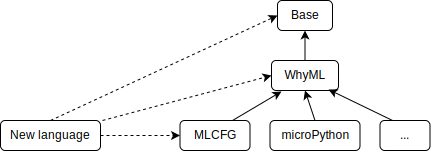
\includegraphics[width=0.5\textwidth]{figs/language_tree.pdf}
    \caption{The default Why3 language tree. \label{fig:langtree}}
\end{figure}

Why3 tracks supported languages in a tree.
Using \inl{Env.register\_language},
plugins can register any arbitrary type as a language
by providing a conversion function to an already-existing language in the tree.
There are two built-in languages that may be targeted for conversion:

\begin{itemize}
    \item \inl{Env.base\_language : Theory.theory Wstdlib.Mstr.t language}\\
          The base language, a dictionary of \inl{theory} values.
    \item \inl{Pmodule.mlw\_language : Pmodule.mlw\_file language}\\
          An internal representation of the WhyML/MLW language.
\end{itemize}

The choice of conversion target depends on our goal.
If the new language can be converted to a WhyML or MLCFG syntax tree,
this will generally be the easier route,
as we can then leverage the power of the existing verification condition generators.
If the language has novel features that require unique VC generation,
we can implement this as a conversion from our language to a theory.
In this project we target the base language,
as this allows us to see how we can use the Why3 framework to build custom VC generators.

Using \inl{Env.register\_format} with a parser and a language handle,
we can register new textual formats for any language.
In fact, the built-in plugins only register new textual formats for MLW.
This is sufficient for most smaller languages such as our While-lang,
but it doesn't create an entry in the language tree,
so a novel language registered this way cannot be a conversion target.

\subsection{Creating formulas}

Logical formulas in Why3 are represented by encapsulated \inl{term} objects,
and are created and modified using combinators from the \inl{Term} module.
The combinators include various constants, predicate logic, function applications,
variable substitutions, and more.
For example, we can create the formula
$\forall x y.~(x \rightarrow y) \leftrightarrow (\neg x \lor y)$
as follows:
\begin{lstlisting}
open Why3
open Term
open Ident

let x  = create_vsymbol (id_fresh "x") in
let y  = create_vsymbol (id_fresh "y") in
let x_var = t_var x in
let y_var = t_var y in
let t1 = t_implies x_var y_var in
let t2 = t_or (t_not x_var) y_var in
let t  = t_forall_close [x; y] [] (t_iff t1 t2)
\end{lstlisting}

Note that identifiers are created using \inl{id\_fresh},
which always creates a unique identifiers.
In order to use the same variable multiple times,
it's necessary to use the exact same identifier everyt time.

Terms and identifiers can also be annotated with locations and attributes using
\inl{Term.t\_set\_attr}.
Position annotations are what enables the Why3 IDE to highlight goals
and subdivided goals after splits.

\subsection{Declarations}

Declarations are made using builder functions located in the module \inl{Term}.
A declaration can be one of:

\begin{itemize}
    \item Abstract types and type aliases
    \item Algebraic data types
    \item Abstract functions and predicates
    \item Defined functions and predicates
    \item Inductive predicates
    \item Propositions:
    \begin{itemize}
        \item Axioms
        \item Lemmas
        \item Goals
    \end{itemize}
\end{itemize}

Theories are primarily built from declarations.
Our small language will translate into a theory with a single goal proposition.

\subsection{Building a \inl{theory}}

All languages are eventually translated into to the base language,
a dictionary of \inl{theory} objects.
A \inl{theory} object is an intermediate representation of a module.
This is the core representation that Why3 can apply transformations to,
convert to SMT queries, and extract code from.

The \inl{theory} type is provided by the \inl{Theory} module,
located in \inl{src/core/theory.mli}.
Theories are created using an encapsulated builder pattern.
Theories ``under construction'' are  created with \inl{create\_theory},
modified using transformers such as \inl{add\_decl},
and finalized using \inl{close\_theory}.

\subsection{Printing}

In addition to parsing,
it is also possible to register a printer for a set of core objects.
This is useful for presenting formulas and tasks in a way that match the syntax of our language.
This is not a strict requirement.

    \section{Implementation} % approx. ? pages. i think i added this point myself.

Our While plugin translates our While language directly to the base language.
Using the previously described weakest precondition calculus,
we generate verification conditions and wrap these in a module as a single proof goal.

We use the Dune build system\cite{dunesite} and require Why3 as a dependency.
Additional dependencies are embedded (statically linked) in the executable,
and we generate both bytecode and a native binary:
\lstinputlisting[lastline=5]{../plugin/lib/dune}

\subsection{Syntax tree}

We define our own AST using zero Why3 dependencies:
\lstinputlisting[lastline=32]{../plugin/lib/wi_ast.ml}
Nodes in this tree are recursively tagged with position information,
with the intent of carrying these annotations through the VC generation.
Aside from this, the only deviation from the grammar in fig. \ref{fig:whilegrammar}
is that sequences are directly defined as lists rather than manual list constructors.

\subsection{Parsing}

For parsing, we use the MParser library\cite{mparser}.
It is a monadic parser combinator library with several useful features.
It lets us avoid the more complex build process
that is necessary in order to use parser generators
(although Dune does seem to have some builtin support for Menhir).
Furthermore, it has documented support for retrieving position information,
which is lacking in other combinator libraries.
Finally, it has a built-in abstraction for parsing expressions with both prefix and infix operators,
operator precedence, and left/right associativity.

Just like with our syntax tree,
the parser is completely independent of the Why3 API as well.
Some utility items are provided by the Why3 API,
but in principle,
both the syntax tree and parser may be defined as we please.
The only strict requirement is that we implement a conversion to another Why3 language.

\subsection{VC-generation}

As we register our own AST as a child of the base language,
we can (and must) perform VC-generation when converting our AST.
Here we implement the weakest precondition calculus described in section \ref{sec:whilewp}.

WP is performed by a recursion on the AST.
There's a lot of legwork to create formulas,
but it's generally a case of matching our WP to the corresponding transformers in the \inl{Term}
module.
In order to support integer arithmetic and comparisons,
we must import the theories \inl{int.Int} and \inl{int.ComputerDivision},
as the base theory only supports equality.
These are provided by the environment to our parser at runtime,
so we must carry the environment as part of our language.

The resulting formula is wrapped in a theory as a proposition goal,
giving us our final base language object.

    \section{Example programs} % approx. 2.5 pages

\subsection{Loop with addition and subtraction}
This program employs an inefficient approach towards moving a value from \inl{a} to \inl{b},
but it provides a demonstration of
a loop invariant, specified preconditions, assignment, arithmetic, and assertions.
It succeeds on both the Z3 and Alt-Ergo provers.
\lstinputlisting{../plugin/examples/add_sub_loop.wi}

%\subsection{}

    \section{Evaluation} % approx. 2 pages

The final product is a clear and well-documented example of a Why3 plugin.
Regrettably, the plugin is not thoroughly tested besides a few simple examples,
so it serves as a demonstration more than anything else.
The greatest limitation of the language and plugin in terms of features
is the lack of functions and predicates.
Another feature that wasn't implemented within the bounds of this project was position annotations,
although the plumbing for this feature is already laid out.
With testing and a few additional features,
the plugin could serve as a great baseline
to which experimental features and their VC generators could be explored.

In this project, we made the choice to convert our AST directly to MLW.
In fact, we could've chosen to register a format parser for MLW
rather than building our own syntax tree.
It might have been simpler and easier to convert our language to MLW instead.
There is nothing in our simple language
that doesn't have a parallel in the rather rich features of WhyML.
However, the API for building MLW syntax trees isn't necessarily simple either.
For a relatively simple language,
implementing a VC-generator is a manageable task.
Choosing to write a conversion also results in a clearer separation of concerns,
making the plugin a good starting point as a template for more advanced plugins.

    \section{Conclusion} % approx .5-1 pages

In this project, we have built a Why3 plugin for a custom language
using our own syntax tree, parser, and verification condition generator.
Along the way, we have explored the theory of the weakest precondition calculus,
documented the necessary parts of the Why3 API,
and shown process of building plugins for Why3.
The supported language is simple and very limited,
but it showcases the possibilities of using Why3
to work directly with languages besides WhyML and MLCFG.


    % use bibtex for references
    % \bibliography{bibliography}
\end{document}
